\chapter{State of the Art}

\section{Hospital Medication Management Systems}

Medication management is a cornerstone of patient safety in hospital environments. The increasing complexity of prescriptions, coupled with the risk of drug interactions, compels healthcare systems to operate with maximum efficiency and safety. In recent years, various solutions have been developed to automate parts of this process, from prescription to administration. However, the lack of integration between these systems—particularly among physicians, pharmacies, and nurses—continues to pose risks and inefficiencies \cite{bowles2020integrating, kallio2020}. This work proposes a solution that addresses these gaps by focusing on backend integration and the automation of hospital processes, using technologies like Java and Node.js to standardize and optimize medication management \cite{Ghobadi2022}.

\subsection{Historical Evolution}

Hospital Information Systems (HIS) have evolved significantly from the early mainframe-based systems of the 1960s. The transition to departmental systems in the 1980s and their subsequent integration via Health Level Seven (HL7) \cite{dolin2006, mandl2020} in the 1990s laid the groundwork for modern systems.

\begin{figure}[htbp]
    \centering
    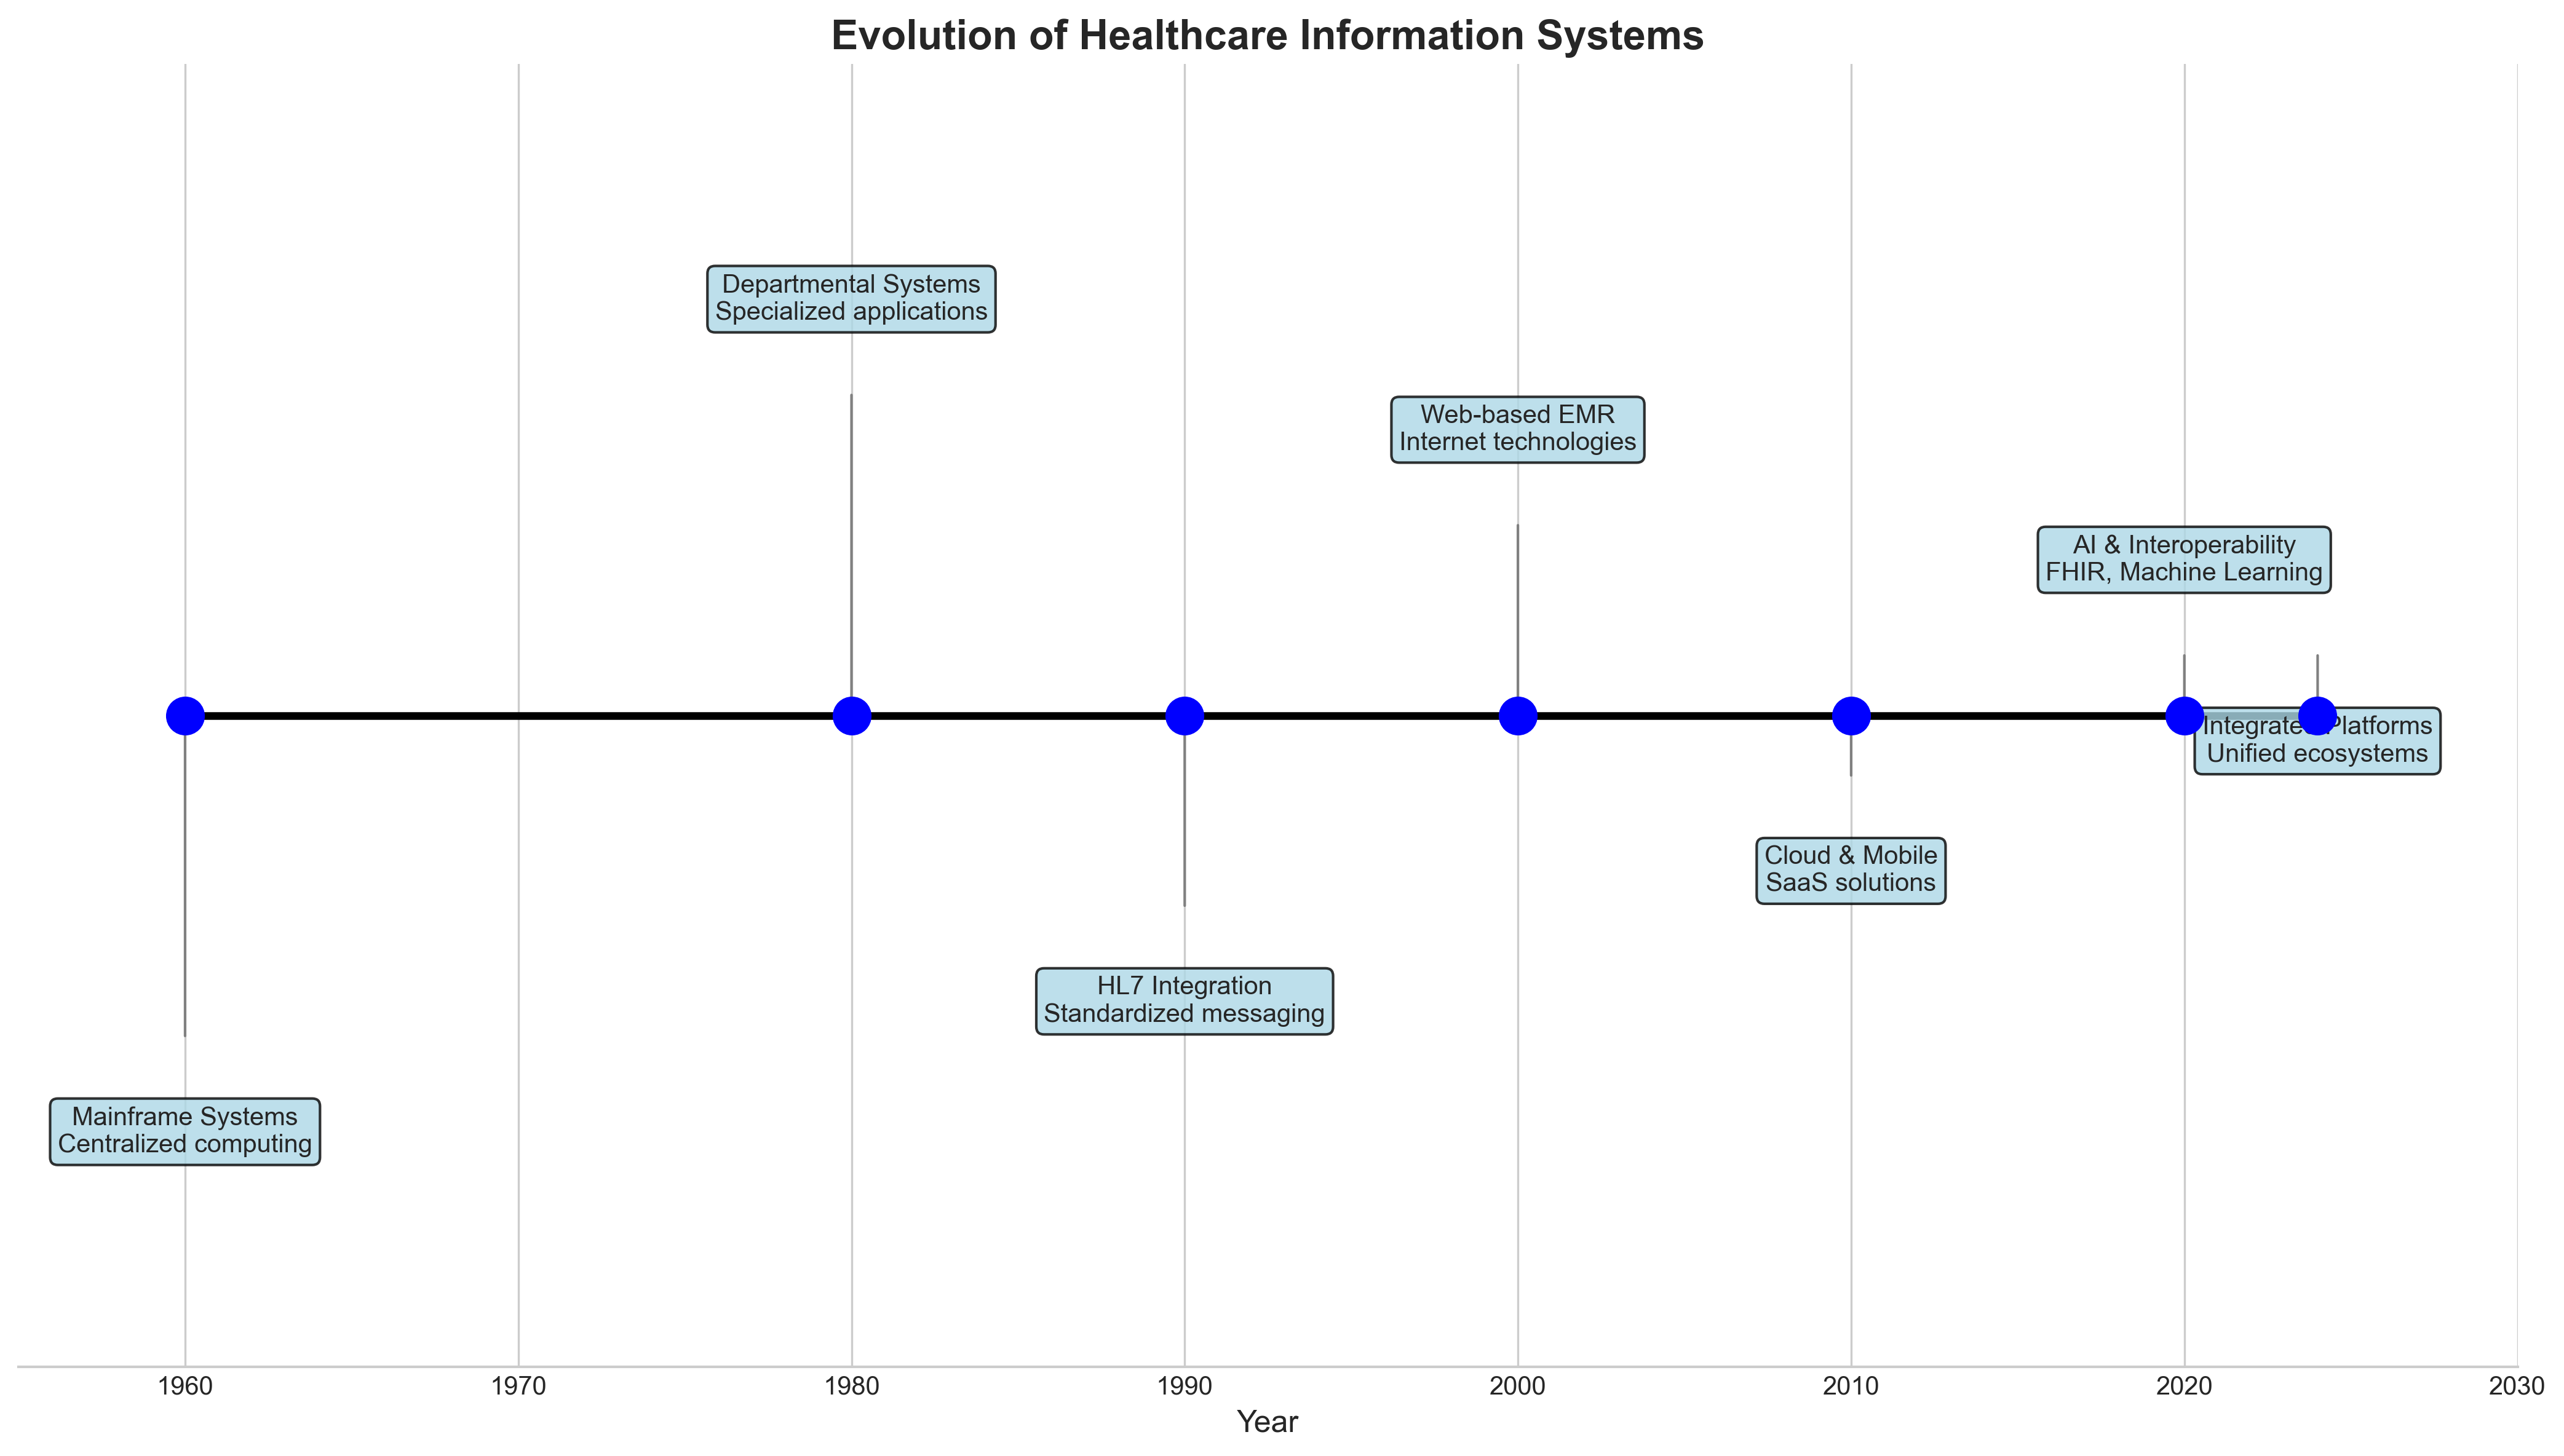
\includegraphics[width=0.95\textwidth]{images/generated/healthcare_it_timeline.png}
    \caption{Evolution of healthcare information systems from mainframe to integrated platforms \citep{shermock2023, vaghasiya2023}.}
    \label{fig:timeline}
\end{figure}

\subsection{Current Commercial Systems}

The current landscape of commercial hospital management systems is dominated by a few key vendors. Epic Systems \cite{hertzum2022} has established itself as a market leader in the United States with its EpicCare system, offering an integrated platform for clinical and administrative management. Cerner, recently acquired by Oracle Health \cite{lin2018}, competes directly with its PowerChart and Millennium solutions. Automated systems like those from Epic aim to ensure that patient data and prescriptions are kept updated and accessible in real-time \cite{keller2023using}. In the European market, InterSystems stands out with TrakCare, which has gained significant acceptance due to its adaptability.

\subsection{Challenges of Current Systems}

Despite technological advancements, current systems face significant challenges. Limited interoperability \cite{keasberry2017} remains a major obstacle, with the lack of effective standards preventing seamless communication between different hospital systems. This fragmentation results in information silos that compromise the continuity of care. Many of these systems operate in a compartmentalized manner, with little to no interoperability among physicians, pharmacists, and nurses, leading to redundancies and risks of human error \cite{Kallio2021}. Furthermore, complex interfaces \cite{mcgreevey2020}, high implementation costs \cite{adler2021}, and resistance to change \cite{holden2011, venkatesh2003} remain significant limiting factors.

\section{Medication Safety and Emerging Technologies}

Medication errors are a leading cause of preventable adverse events in healthcare \cite{ciapponi2021, mulac2020}. These errors can occur at any stage of the medication process, including prescribing, transcribing, dispensing, and administration \cite{isaacs2021, manias2021, kallio2020, boytim2018}. The Swiss Cheese Model is often used to illustrate how these failures can align to cause harm \citep{ciapponi2021, mulac2020}.

\begin{figure}[htbp]
    \centering
    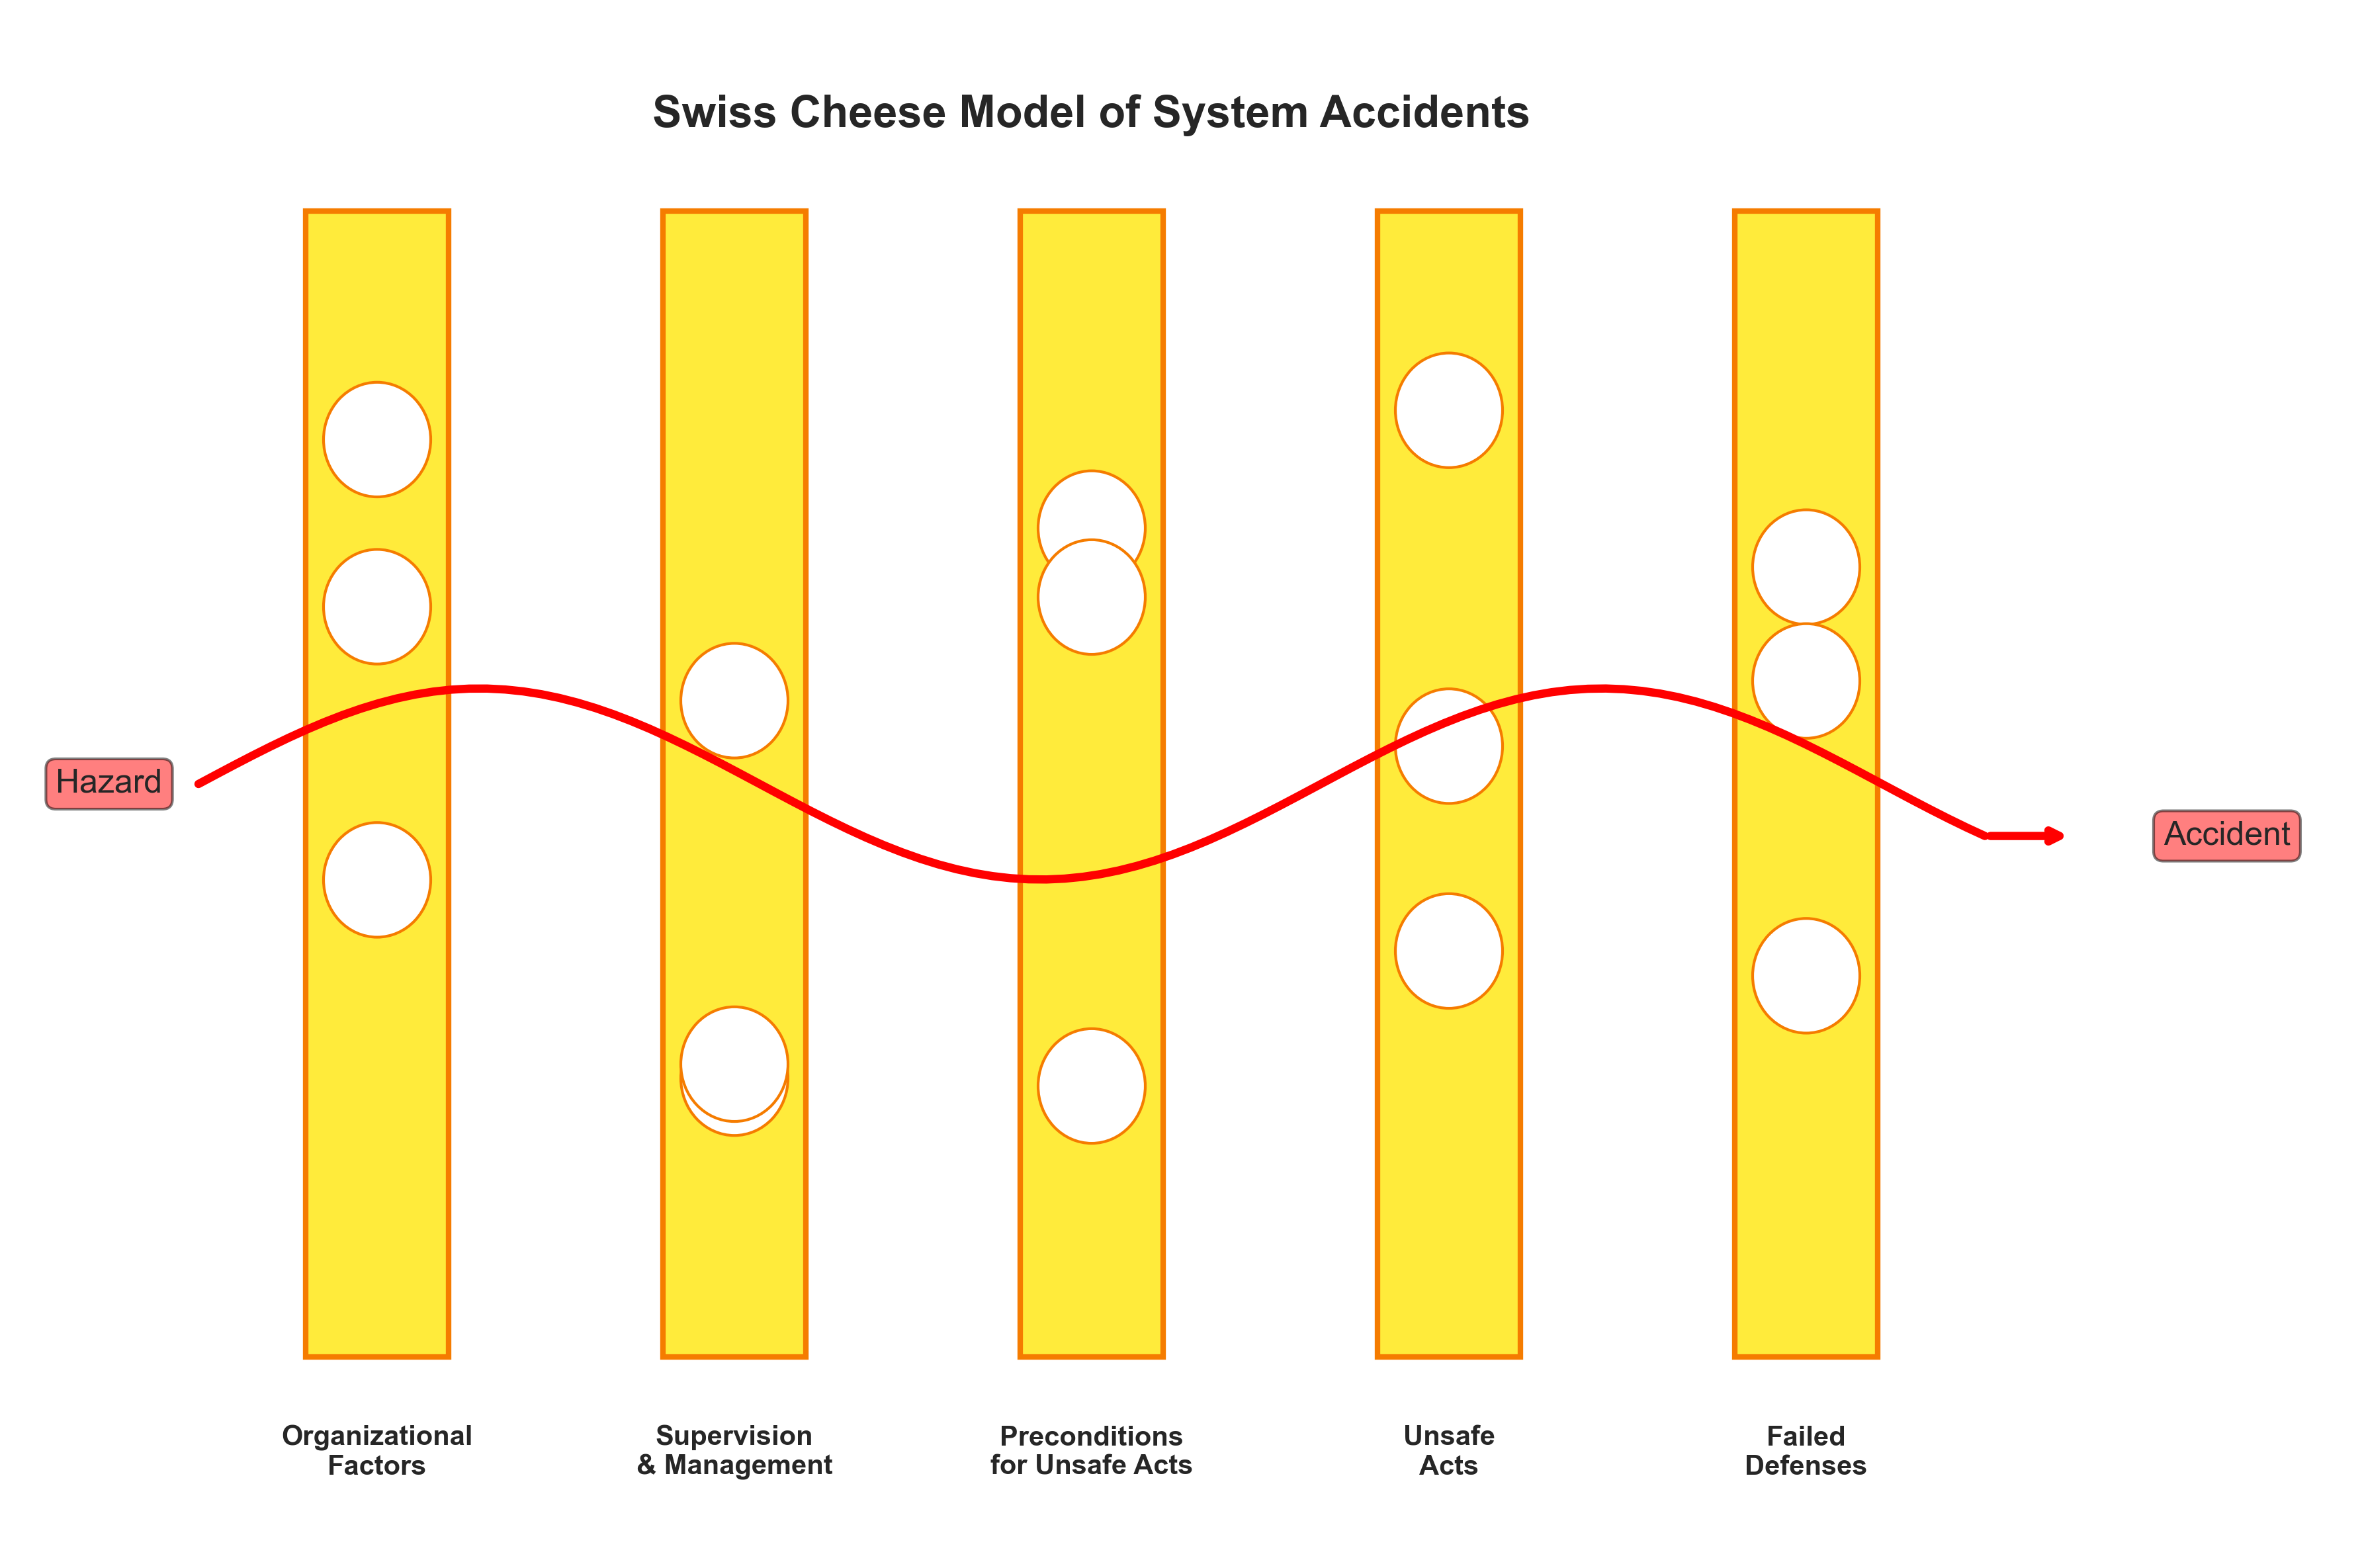
\includegraphics[width=0.85\textwidth]{images/generated/swiss_cheese_model.png}
    \caption{Swiss Cheese Model applied to medication errors, showing how system failures align to cause accidents. Based on Reason's model \citep{ciapponi2021, mulac2020}.}
    \label{fig:swiss_cheese}
\end{figure}

\subsection{Clinical Decision Support Systems (CDSS)}

Clinical Decision Support Systems (CDSS) \cite{moss2015, belle2013} and ePrescribing systems have been widely implemented to minimize medication errors \cite{belle2013biomedical, hawley2019}. However, the lack of integration between these modules remains a significant problem. Modern CDSS incorporate features such as real-time interaction checks, guideline-based alerts, and machine learning for personalization \cite{bates2021, zhao2021}.

\subsection{Artificial Intelligence in Healthcare}

The application of Natural Language Processing (NLP) \cite{rozenblum2020} is particularly relevant for extracting drug-drug interaction (DDI) information from unstructured biomedical texts \cite{javaid2022medical}. Systems like the one proposed by Machado \textit{et al.} (2023) use NLP to automatically extract DDI information from scientific literature \cite{machado2023drug}. Tools such as BioBERT have shown promise in this area \cite{Russell2023}. However, low interoperability rates and the absence of universal standards still hinder the widespread adoption of these technologies \citep{Chaya2023}. The development of APIs that can seamlessly integrate data from various hospital systems with NLP and AI platforms is a promising area for further exploration \cite{López2021}.

\subsection{Other Emerging Technologies}

Other technologies like Blockchain also show promise for enhancing medication traceability, decentralized consent management, and immutable auditing of prescriptions \cite{franzoso2014}.

\section{Implementation Architectures and Technologies}

Despite significant advances in hospital process automation, several technical challenges must be overcome. Integrating legacy systems with new technologies requires the standardization of programming languages and communication protocols \cite{stanojevic2023conceptualizing}. Technologies such as Java and Node.js are widely used in backend solutions to ensure scalability, resilience, and data security in critical environments \cite{nkenyereye2016performance}. Furthermore, the complexity of hospital workflows demands automation that transcends mere data exchange. Real-time synchronization between physician prescriptions, pharmacy stock, and nursing administration is crucial to avoid medication errors, particularly in cases of polypharmacy \citep{Tukukino2022, falconer2021pharmacist}.

\subsection{Architectural Patterns}

Microservices architecture offers several advantages for hospital systems, including independent scalability, resilience to failures, and easier integration with legacy systems \cite{shermock2023, vaghasiya2023, newman2021}. This is often implemented alongside established integration patterns. An API Gateway can serve as a single entry point for all client requests \cite{newman2021}, while a Service Mesh can manage inter-service communication. Adopting an event-driven architecture facilitates asynchronous communication \cite{fowler2018}, and patterns like CQRS (Command Query Responsibility Segregation) can help manage data complexity by separating read and write operations.

\subsection{Standards and Interoperability}

Standards are crucial for achieving interoperability. HL7 FHIR (Fast Healthcare Interoperability Resources) represents the evolution of the HL7 standard, offering native RESTful APIs, modular resources, and support for mobile applications, making it a key enabler for modern, integrated healthcare systems.

\section{Gaps and Opportunities}

The literature review reveals several gaps in existing solutions. The most significant is deficient integration, as current systems often fail to provide seamless interoperability among stakeholders, leading to information silos. This is compounded by usability issues, where interfaces are not optimized for clinical workflows. This dissertation addresses these gaps by proposing a solution centered on a non-invasive integration architecture, user-centered design, and an incremental implementation model. The use of a centralized backend to orchestrate all processes, from prescription to administration, presents a key opportunity to create a single source of truth and bridge these gaps.

\begin{table}[H]
    \centering
    \caption{Comparative analysis of hospital medication management systems including legacy and modern solutions.}
    \label{tab:comparison}
    \begin{tabularx}{\textwidth}{@{}l|X|X|X|X@{}}
        \toprule
        \textbf{Feature} & \textbf{AIDA-PCE (Legacy)} & \textbf{Epic} & \textbf{Cerner} & \textbf{Our System} \\
        \midrule
        Architecture & Monolithic & Integrated Suite & Modular & Microservices \\
        User Interface & Desktop Only & Web/Mobile & Web/Mobile & Responsive Web \\
        Real-time Validation & Limited & Yes & Yes & Advanced \\
        Integration & Custom APIs & HL7/FHIR & HL7/FHIR & RESTful/HL7 \\
        Cloud Support & No & Hybrid & Yes & Cloud-Ready \\
        Cost Model & License & Subscription & Subscription & Open Source \\
        Customization & Limited & Moderate & High & Very High \\
        AI/ML Features & None & Basic & Advanced & Planned \\
        \bottomrule
    \end{tabularx}
\end{table}

\section{Conclusion and Positioning}

The review of the state of the art reveals that despite significant technological advances, a critical gap persists in the interoperability and integration of medication management systems. This work is positioned to address this gap directly. It puts forward a validated model for modernizing hospital workflows through a non-invasive integration strategy, demonstrating that it is possible to create a single, cohesive source of truth without completely replacing legacy infrastructure.

The decision to use enterprise-grade technologies like Java and Node.js was a direct response to the need for secure, scalable, and resilient systems capable of operating in a mission-critical hospital environment. By focusing on a robust backend that orchestrates the entire medication lifecycle, this dissertation presents a pragmatic yet powerful solution to enhance patient safety, improve operational efficiency, and bridge the integration gaps that characterize modern healthcare IT. 